\chapter[P2: A Logical Beginning]{P2: A Logical Beginning}
\label{ch:p2}

This chapter contains background material related to the {\em Declarative
Networking} project~\cite{boon-thesis}, which is a lead-in to this thesis.  The
original project members included Boon Thau Loo, Tyson Condie, Joseph M.
Hellerstein, and Ion Stoica at the {\em University of California, Berkeley},
Petros Maniatis and Timothy Roscoe at {\em Intel Research Berkeley}, and Raghu
Ramakrishnan at {\em Yahoo!  Research}.  Together, we developed a new
declarative language called {\em \OVERLOG} and a runtime system called {\em
P2}.  Our initial goal was to make it easy to implement and deploy {\em
overlay} networks~\footnote{A computer network built on top of an existing
network e.g., IP (layer 3).} by allowing specifications in a high-level
declarative language to be directly executed on nodes that span the Internet.
These overlay specifications, expressed as \OVERLOG rules, contained {\em
orders of magnitude} fewer lines of code than the corresponding overlay
implementations written in an imperative language (e.g., C/C++).  The project
implemented, and deployed, declarative versions of a Narada-style mesh
network~\cite{chu00case}, using only 12 ``rules'', and the Chord structured
overlay~\cite{chord} in only 35 ``rules''~\cite{p2:sosp}.  The P2 project
clearly showed that relations, together with a recursive query language, can
fairly naturally represent the persistent routing state of the overlays it
considered~\cite{boon-thesis}.

The \OVERLOG language is a descendent of Datalog, which we review in
Chapter~\ref{ch:p2:sec:datalog}.  In Chapter~\ref{ch:p2:sec:overlog}, we
present the \OVERLOG language by detailing its extensions to Datalog: it adds a
notation to specify the location of data, provides some SQL-style extensions
such as primary keys and aggregation, and adds a flexible notion of state
lifetime.  Chapter~\ref{ch:p2:sec:p2} describes the P2 runtime, which is
responsible for compiling and executing \OVERLOG programs on a set of
distributed nodes.  The design of P2 was inspired by prior work in both
databases and networking.  It is based in large part upon a side-by-side
comparison of the PIER peer-to-peer query engine~\cite{pier-cidr05} and the
Click modular router~\cite{click-tocs}.  Like PIER, P2 can manage structured
data tuples flowing through a broad range of query processing elements, which
may accumulate significant state and perform substantial asynchronous
processing.  Like Click, P2 stresses high-performance transfers of data units,
as well as dataflow elements with both ``push'' and ``pull'' modalities.

\section{Introduction to Datalog}
\label{ch:p2:sec:datalog}

Our description of Datalog is based on a survey by Ramakrishnan and
Ullman~\cite{deductive-database}, and course notes~\cite{ullmanNotes} on the
subject.  Datalog drew inspiration from the Prolog language, which was one of
the first logic programming languages.  Both Datalog and Prolog consist of a
set of declarative {\em rules} and an optional {\em query}.  A rule has the
form $p\ \text{\ol{:-}}\ q_1,\ q_2,\ \ldots,\ q_n$, which informally reads
``{\bf if} $q_1$ and $q_2$ and $\ldots$ and $q_n$ is true {\bf then} $p$ is
true.'' The predicate appearing to the left of the \ol{:-} symbol is the head
predicate, and those to the right are body literals or ``subgoals.'' Literals
are either {\em predicates} over {\em fields} (variables and constants), or
function symbols applied to fields.  Recursion is expressed by rules that refer
to each other in a cyclic fashion.  That is, the head predicate also appears as
a subgoal in the rule, or indirectly through some other subgoal predicates.

A predicate literal is a named reference to a set of data tuples associated
with a specific schema.  In Datalog, a data tuple is referred to as a {\em fact},
which is stored in a relational table that may not necessarily fit in memory.
A predicate whose relation is stored in the database is called an {\em
extensional database} (EDB) relation, while those that are defined by logical
rules are called {\em intensional database} (IDB) relations.  In other words,
EDB tuples are those that persist in the database as relations, while IDB
predicates are more like ``views'' (or stored queries) over the database
schema.

During evaluation, EDB facts represent the input to the Datalog program, and
IDB derivations are the output.  Most implementations of Datalog evaluate rules
in a bottom up fashion, starting with all known EDB facts, and deriving new IDB
facts through rule deductions.  A key consequence of a bottom-up evaluation
strategy is that it can efficiently handle relations whose size exceed the
capacity of a machine's main memory.

%Prolog on the other hand uses
%a top-down evaluation approach that precludes the efficient use of relational
%operators (i.e., select, project, join).  As a further result, Prolog's state
%is confined to the main memory boundaries of the running system, since its
%``graph'' based algorithm requires all facts be accounted for at once.

\subsection{Datalog Syntax}

\begin{figure*}
\ssp
\begin{lstlisting}
link(``node1'', ``node2'', 1).
link(``node2'', ``node3'', 1).

r1 path(X, Y, cons(X, Y), C) :- 
   link(X, Y, C). 

r2 path(X, Z, cons(X, P2), C1+C2) :- 
   link(X, Y, C1), path(Y, Z, P2, C2),
   contains(X, P2) == false.

query path(``node1'', Y, P, C).
\end{lstlisting}
\caption{\label{ch:p2:fig:datalogPath}Path program written in Datalog.}
\end{figure*}

Figure~\ref{ch:p2:fig:datalogPath} provides our first look at a program
expressed in Datalog.  The {\em fact} statements at the top specify the
existence of two data tuples in the \ol{link} table with the given attribute
constants.  Each row of the \ol{link} table contains three attributes; two
strings, and an integer.  The program rules derive all reachable paths from
this initial set of known \ol{link} tuples, and presents that result in a
relational view called \ol{path}.

Base derivations proceed from the rule body (those predicates to the right of
``\ol{:-}'') and project onto the rule head (to the left of ``\ol{:-}'').  The
\ol{link} facts are used in the evaluation of rule~\ol{r1} to derive an initial
set of \ol{path} tuples.  The rule reads ``if there exists a \ol{link} from $X$
to $Y$ at cost $C$, then there exists a \ol{path} from $X$ to $Y$ consisting of
nodes $X, Y$ at cost $C$.'' Both initial facts meet this criterion and hence
are included in the \ol{path} relation.

Rule~\ol{r2} expresses a transitive closure over the \ol{link} and \ol{path}
relations.  The rule reads ``if there is a link from $X$ to $Y$ at cost $C$,
and there is a \ol{path} $P2$ from $Y$ to $Z$ at cost $C2$, then there is a
path from $X$ to $Z$ via $P2$ at cost $C1+C3$.'' A path from ``node1'' to
``node3'', through ``node2'', satisfies this criterion, and such a tuple is
included in the \ol{path} IDB relation.  The selection predicate
\ol{contains(X, P2) == false} avoids cyclic paths to ensure a finite result and
program termination.  The ``query'' predicate at the bottom of
Figure~\ref{ch:p2:fig:datalogPath}, asks for all paths that start at ``node1.''
The \ol{path} tuples that begin with ``node1'' and end at ``node2'' and
``node3'' (via ``node2'') both meet this query constraint.

\subsection{Safety First}
\label{ch:p2:sec:safety}

There are constraints that must be in place for a Datalog program to make sense
as operations on finite relations.  
\begin{mydef}
\ssp
A {\em safe} Datalog rule ensures that all variables mentioned in the rule
appear in some nonnegated subgoal table predicate of the rule body.
\end{mydef}
This definition ensures that all variables in negated subgoals and the head
predicate are restricted by some nonnegated subgoal table predicate.  For example,
the following rule is not safe since it does not restrict the $P$ variable in
the \ol{path} head predicate.
\begin{lstlisting}[frame=none]
path(X, Y, P, C) :- link(X, Y, C).
\end{lstlisting}
The above rule generates an infinite number of \ol{path} tuples since we can
substitute any conceivable value for $P$.  A safe Datalog rule is a necessary,
but not sufficient,~\footnote{The programmer can still express an infinite
solution i.e., by leaving out \ol{contains(X,~P2)~==~false} in rule~\ol{r2}}
condition to obtaining a finite (IDB) solution from evaluating a finite set of
rules on a finite (EDB) input.  Datalog further restricts its (IDB) output to
set semantics, as opposed to bag semantics that allow duplicate tuples.  The
reader can assume these safety restrictions in all the rules presented in this
thesis.

\subsection{Evaluation of Datalog Rules}
\label{ch:p2:sec:eval}

We now turn to the evaluation of a set of Datalog rules, which is performed in
a bottom-up fashion, starting with the set of known EDB facts.  There are two
standard approaches to evaluating a set of Datalog rules.  The first is called
{\em na\"{\i}ve evaluation}, which is an iterative algorithm that repeatedly
applies all known facts to the program rules, in some stylized set-oriented
fashion, until no new knowledge is obtained.  Starting with the tuples
contained in the EDB, the na\"{\i}ve evaluator iteratively executes a
select-project-join (SPJ) query against the predicates in the rule body, to
continually derive new IDB tuples.  Each iteration applies all the tuples
contained in the EDB and IDB to the rule set.  The process repeats until no new
tuples can be inferred, marking the end of the evaluation, which is commonly
referred to as a ``fixed point.''

Each iteration of this na\"{\i}ve algorithm uses all known data in the database
when deriving new data.  A second approach, which is also the optimal approach,
adds a condition to the iteration loop that prunes the data that was not
derived in the previous round.  The remaining facts, if any, are then used in
the subsequent iteration.  This {\em semina\"{\i}ve evaluation} algorithm is
based on the principle that ``if a fact is derived during round~$i$ then it
must have been inferred from a rule in which one or more subgoals were
instantiated with facts that were inferred in round~$i-1$.''~\cite{ullmanbook}


\begin{figure*}
\ssp
\begin{boxedminipage}{\linewidth}
    \begin{algorithmic}[1]
      \STATE \ol{path} = $\Delta$\ol{path} = $\pi_{X, Y, cons(X, Y), C}$\ol{link}
      \WHILE{$\Delta$\ol{path}\ !=\ $\emptyset$}
      	\STATE $\Delta$\ol{path} = $\pi_{X,\ Z,\ cons(X, P2),\ C1+C2}$ 
      	($\sigma_{contains(X,P2)\ ==\ false}$(\ol{link} $\Join$ $\Delta$\ol{path})) 
      	\STATE $\Delta$\ol{path} = $\Delta$\ol{path} - \ol{path}
      	\STATE \ol{path} = \ol{path} $\bigcup$ $\Delta$\ol{path}
      \ENDWHILE
    \end{algorithmic}
\end{boxedminipage}
\caption{\label{ch:p2:fig:seminaive}Semina\"{\i}ve evaluation of the 
path program in Figure~\ref{ch:p2:fig:datalogPath}.}
\end{figure*}

Figure~\ref{ch:p2:fig:seminaive} describes the steps performed by a
semina\"{\i}ve evaluation of the path program shown in
Figure~\ref{ch:p2:fig:datalogPath}.  $\Delta$\ol{path} references
the set of new tuples added to the \ol{path} relation in the previous round.
In round one, line~$1$ of the algorithm uses rule~\ol{r1} to derive the initial
set of \ol{path} tuples from the EDB \ol{link} relation.  Subsequent rounds are
carried out in the \ol{while} loop (lines $2 \cdots 6$) until $\Delta$\ol{path}
is empty.  The body of the loop contains the following three steps.
\begin{enumerate} \ssp 
  \item Evaluate rule~\ol{r2} relative to the tuples in
    $\Delta$\ol{path}.  
  \item Assign $\Delta$\ol{path} to the new tuples
    derived in this round only.  
  \item Accumulate the new $\Delta$\ol{path} in the \ol{path} relation.  
\end{enumerate}

In the first step, we evaluate rule~\ol{r2} using the $\Delta$\ol{path} tuples
derived in the previous round (e.g., initially, those obtained from the
\ol{link} relation).  In general, if there existed other rules that referenced
\ol{path} in the body, then those too would be evaluated against the same
$\Delta$\ol{path} tuples, and any deductions would contribute to the $\Delta$
predicate referenced by the rule head.  The last two steps in the loop deal
with ensuring $\Delta$\ol{path} only references deductions from the previous
round, and that the new deductions are accumulated in the \ol{path} relation.


\subsection{Fixed Point Semantics}

Datalog is a monotonic language: once a fact is derived during evaluation it is
certain to be in the final answer.  The evaluation of a program proceeds as a
series of deductions to the IDB.  A Datalog program is said to be at a {\em
fixed point} when no further deductions can be made relative to the current EDB
and IDB tuples.  The result derived at a fixed point is a model for the Datalog
program.  Given a model~$m$ and a Datalog program~$p$, $m$ is a minimal model
if and only if no proper subset of $m$ is a model for $p$.  In the absence of
negated subgoals, a Datalog program has one and only one minimal model.  A
logic program with negation may have more than one minimal model. However, if
the program is ``stratified'' then there is a uniquely identifiable
``intended'' minimal model, based on the (stratification) order in which the
relations are (intended to be) minimized.~\cite{deductive-database}


\subsection{Negation and Stratification}

We touch on the subject of handling negated subgoals in the body of a Datalog
rule.  There is a large body of work on this subject that we will not address
here since it does not pertain to the content of this thesis.  Our goal instead
is to introduce the reader to the notion of stratified negation, which ensures
that a set of Datalog rules with negated subgoals ``make sense'', by way of
reaching a unique minimal model on a fixed point evaluation.  Before going
further, we review some semantic issues raised by negated subgoals in Datalog.

\begin{figure*}
\centering
\ssp
\begin{lstlisting}
r4 path(X, Y, P, C) :-
   link(X, Y, C),
   not detour(X, Y).

r5 detour(X, Y) :-
   link(X, Y, C),
   ... 
\end{lstlisting}
\caption{\label{ch:p2:fig:negation}Negated Datalog rule.}
\end{figure*}

Consider rule~\ol{r4} in Figure~\ref{ch:p2:fig:negation}, which formulates a
\ol{path} from a \ol{link} if $X$ and $Y$ does not cross a detour.
Unfortunately, the complement of the \ol{detour} relation is not well-defined
since the variables range over an infinite domain the compliment is also
infinite.  Moreover, we cannot specify this complete relation prior to
evaluation, since \ol{detour} is an IDB predicate.  If we were to simply
evaluate the rules in Figure~\ref{ch:p2:fig:negation} (using for example the
semina\"{\i}ve algorithm) then we could end up with \ol{path} tuples that cross
detours.  To see this, lets assume that we start by evaluating rule~\ol{r4}
with the initial facts in the \ol{link} relation.  The execution plan for the
negated \ol{detour} is similar to an anti-join operation, where tuples from
\ol{link} relation pass if they do not already exist in the current \ol{detour}
relation.  Since we have not yet evaluated rule~\ol{r5}, all \ol{link} tuples
pass the anti-join, and produce a set of \ol{path} deductions in rule~\ol{r4}.
Subsequently evaluating rule~\ol{r5} would give us our \ol{detour} tuples, but
this would be too late in the sense that we have already made incorrect
deductions, and cannot take them back.

\begin{figure*} 
\ssp
\begin{center}
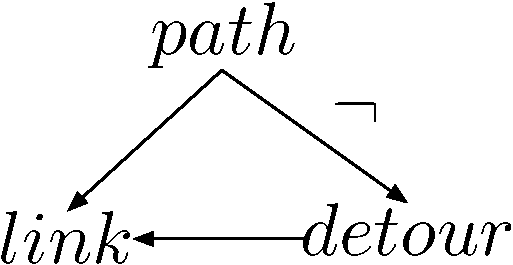
\includegraphics[scale=0.75]{figures/dependency-graph}
\caption{\label{ch:p2:fig:dependency}Dependency graph for predicates 
appearing in Figure~\ref{ch:p2:fig:negation}.}
\end{center} 
\end{figure*}

We could obtain the correct IDB by simply evaluating rule~\ol{r5} first.  Such
an ordering of predicate evaluations forms the basic idea behind stratified
Datalog.  Before we get to that definition, we first review how the
dependencies of a Datalog program are represented graphically.
Figure~\ref{ch:p2:fig:dependency} contains the dependency graph for the
predicates appearing in the rules of Figure~\ref{ch:p2:fig:negation}.
Constructing this graph is a straightforward application of the following two
rules.
\begin{enumerate}
  \ssp
  \item Add $p \rightarrow q$ dependency if there is a rule with head predicate $p$ and subgoal $q$.
  \item Add $p \rightarrow q$ dependency labeled $\neg$ if there is a rule with head predicate $p$ and negated subgoal $q$.
\end{enumerate}
From Figure~\ref{ch:p2:fig:negation}, rule~\ol{r4} forms the $path \rightarrow
link$ and $path \rightarrow detour$ dependencies, while rule~\ol{r5} supplies the
$detour \rightarrow link$ negated edge dependency. 

The stratum of an IDB predicate $p$ is defined to be the largest number of
negations ($\neg$) along any path involving predicate $p$.  The dependency graph
in Figure~\ref{ch:p2:fig:dependency} places predicates \ol{detour} and
\ol{link} in the lowest stratum~$0$, while the \ol{path} predicate is in
stratum~$1$.  If all IDB predicates have a finite stratum, then the Datalog
program is {\em stratified}.  If any IDB predicate has an $\infty$ stratum,
then the program is unstratified.  An IDB predicate is assigned an $\infty$
stratum if it defines a negated subgoal on a path that contains a cycle (due
to arbitrary recursion).

We evaluate a stratified Datalog program using the semina\"{\i}ve algorithm
(e.g., Figure~\ref{ch:p2:fig:seminaive}) but with a slight twist -- we sort the
IDB predicates by their assigned stratum, and follow this order when choosing
$\Delta$ predicates (e.g., $\Delta$ \ol{path}) to evaluate in the loop.  This
order ensures that if the program is stratified then any negated subgoal (e.g.,
\ol{detour}) has already had its relation fully evaluated first.  The result of
this evaluation is called a {\em stratified model}~\footnote{We further note
that the notion of stratified Datalog has nothing to do with the termination of
a Datalog program.  The issue here is the existence a unique minimal result
that is consistent with the programmer's intent.}.

We revisit the notion of stratified Datalog throughout this thesis.  It turns
out that the P2 system does not supported stratified Datalog, which slightly
complicated the (\OVERLOG) program rules described in Chapters~\ref{ch:evita},
\ref{ch:magic} and~\ref{ch:opt}.  Fortunately, there is another class of {\em
locally stratified} Datalog programs that ``make sense'' on certain data.

\subsection{Local Stratification}

Stratified Datalog is defined in terms of a syntactic property that translates
to cycles through negations in the dependency graph of a collection of rules.
An extension to this definition is a class of locally stratified programs,
which is defined in terms of a data dependent property.  Intuitively, these
programs are not necessarily stratified according to their rules, but they are
stratified when we instantiate those rules on a specific collection of data.
Many of the programs presented in this thesis fall into the class of locally
stratified rules.

\begin{figure*}
\ssp
\begin{lstlisting}
link(``node1'', ``node2'', 1).
link(``node2'', ``node3'', 1).

r1 path(X, Y, cons(X, Y), C) :-
   link(X, Y, C).

r2 path(X, Z, cons(X, P2), C1+C2) :-
   link(X, Y, C1), shortestPath(Y, Z, P2, C2),
   contains(X, P2) == false.

r3 minCostPath(X, Y, min<C>) :-
   path(X, Y, P, C).

r4 shortestPath(X, Y, P, C) :-
   minCostPath(X, Y, C), path(X, Y, P, C).

\end{lstlisting}
\caption{\label{ch:p2:fig:datalogSP}Shortest path variant of Figure~\ref{ch:p2:fig:datalogPath}.}
\end{figure*}

Like negation, an aggregation adds a stratification boundary to a Datalog
program.  Intuitively, we must derive all facts from the tables mentioned in
the rule body, before we can evaluate the aggregate in the rule head.
Consider the variant of the path program in Figure~\ref{ch:p2:fig:datalogSP},
which modifies rule~\ol{r2} to formulate new paths from the \ol{shortestPath}
relation, rather than the \ol{path} relation.  Two extra rules \ol{r3} and
\ol{r4} are used to derive the shortest path from the \ol{path} relation.
Rule~\ol{r3} selects the minimum cost path from $X$ to $Y$, and rule~\ol{r4}
selects the actual minimum path based on the minimum cost value in $C$.

\begin{figure*} 
\ssp
\begin{center}
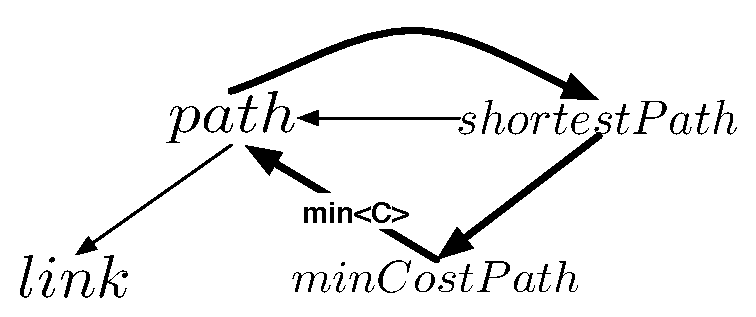
\includegraphics[scale=0.75]{figures/dependency-graph2}
\caption{\label{ch:p2:fig:dependency2}Dependency graph for predicates 
appearing in Figure~\ref{ch:p2:fig:datalogSP}. A cycle through an aggreagation
appears in bold. }
\end{center} 
\end{figure*}

The dependency graph for this program is shown in
Figure~\ref{ch:p2:fig:datalogSP}.  As shown, this program is not stratified
since there is a cyclic path in the rule dependency graph that traverses an
aggregation.  Intuitively, we need to derive all \ol{path} tuples before we can
identify the one that is of minimum cost.  Yet, \ol{path} derivations are based
on what ``currently'' exists in the \ol{shortestPath} relation.  As a result,
the Datalog program in Figure~\ref{ch:p2:fig:datalogSP} is not stratified.

It is however locally stratified.  Assume that this program is evaluated using
the semina\"{\i}ve algorithm (e.g., Figure~\ref{ch:p2:fig:seminaive}).  The
only option in the first step of the bottom-up evaluation is to derive all
paths of length $1$ using rule~\ol{r1}.  Subsequent steps recursively use
rule~\ol{r2} to derive paths of length $2, 3, \ldots$ (fully, in that order)
until no further paths exist.  These derivations are monotonic because we are
performing a {\em min} aggregation of a {\em sum} over non-negative integers.
As a result, rule evaluations derive \ol{path} tuples of length $k$ before path
tuples of length $j > k$, which ensures that new \ol{path} tuples are derived
from a (seemingly) complete set of \ol{shortestPath} tuples.

Many of the programs described in this thesis are not stratified, and of those,
all are locally stratified.  For example, the System R rules presented in
Chapter~\ref{ch:opt} performs a {\em min} aggregation on the cost~\footnote{ A
non-negative integer value.} of a query plan.  This is used to select the
``best plan'' among the set of equivalent plans in a given level (plan size) of
the System R dynamic program.  The ``best plan'' is then recursively used to
construct new plans, containing an extra predicate, for the next dynamic
programming level~\footnote{Each level of the System R dynamic program adds an
extra predicate to the query plan.}.  Since adding an extra predicate to a
query plan can only increase its cost ({\em principle of optimality}), and we
fully explore all plans in a given level before moving to the next, this
optimization is locally stratified.


\section{\OVERLOG: Our first look}
\label{ch:p2:sec:overlog}

\OVERLOG marks a new beginning for the Datalog recursive query language, where
distribution through data partitioning takes center stage.  Like Datalog, an
\OVERLOG~{\em program} consists of a set of deduction {\em rules} that define
the set of tuples that can be derived from a base set of tuples called {\em
facts}.  Each rule has a {\em body} on the right of the \texttt{:-} divider,
and a {\em head} on the left; the head represents tuples that can be derived
from the body.  The body is a comma-separated list of {\em terms}; a term is
either a {\em predicate} (i.e., a relation), a {\em condition} (i.e., a
relational selection) or an {\em assignment}~\footnote{\OVERLOG's assignments
are strictly syntactic replacements of variables with expressions; they are
akin to ``\#define'' macros in C++.}.  An example \OVERLOG program is shown in
Figure~\ref{ch:p2:fig:overlogSP}.  \OVERLOG introduces some notable extensions
to Datalog, which we describe before presenting the P2 runtime.

\begin{figure*}
\ssp
\begin{lstlisting}
materialize(link, infinity, infinity, keys(1,2)).
materialize(path, infinity, infinity, keys(1,2,3)).
materialize(shortestPath, infinity, infinity, keys(1,2,3)).

link(``localhost:10000'', ``localhost:10001'', 1).
link(``localhost:10001'', ``localhost:10002'', 1).

r1 path(@X, Y, P, C) :-
   link(@X, Y, C), P := f_cons(X, Y).

r2 path(@X, Z, P, C) :-
   link(@X, Y, C1), path(@Y, Z, P2, C2),
   f_contains(X,P2) == false,
   P := f_cons(X,P2), C := C1 + C2.

r3 minCostPath(@X, Y, a_min<C>) :-
   path(@X, Y, _, C).

r4 shortestPath(@X, Y, P, C) :-
   minCostPath(@X, Y, C), 
   path(@X, Y, P, C).

query shortestPath(``localhost:10000'', Y, P, C).
\end{lstlisting}
\caption{\label{ch:p2:fig:overlogSP}Shortest path program in \OVERLOG. We
follow the notation of Loo et al.~\cite{boon-thesis}: \ol{a\_}
prefixes introduce aggregate functions and \ol{f\_} prefixes introduce
built-in functions. Variables that do not contribute to the rule evaluation
are ignored using an underscore e.g., rule~\ol{r3}, third \ol{path} attribute.
We will use '$\ldots$' to indicate a series of ignored variables. }
\end{figure*}

\subsection{Horizontal partitioning}

\OVERLOG's basic data model consists of relational tables that are partitioned
across distributed nodes in a network.  Each relation in an \OVERLOG rule must
have one attribute, whose variable is preceded by an ``@'' sign.  This
attribute is called the {\em location specifier} of the relation, and must
contain values in the network's underlying address space (e.g., IP addresses
for Internet settings, 802.13.4 addresses for sensor networks, hash-identifiers
for code written atop distributed hash tables, etc.).  Location specifiers
define the horizontal partitioning of the relation: each tuple is stored at the
address found in its location specifier attribute.  At a given node, we call a
tuple a {\em local tuple} if its location specifier is equal to the local
address.  Network communication is implicit in \OVERLOG: tuples must be stored
at the address in their location specifier, and hence the runtime engine has to
send some of its derived tuples across the network to achieve this physical
constraint.  Loo, et al.  provide syntactic tests to ensure that a set of rules
can be maintained partitioned in a manner consistent with its location
specifiers and network topology~\cite{loo-sigmod06}.


\subsection{Soft State and Events}

\begin{figure*} 
\ssp
\begin{center}
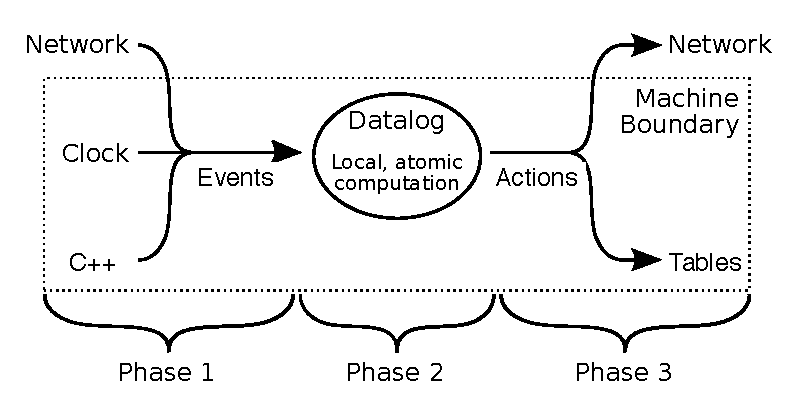
\includegraphics[scale=0.75]{figures/event_loop}
\caption{\label{ch:p2:fig:fixpoint}A single \OVERLOG fixpoint.}
\end{center} 
\end{figure*}

The three phases shown in Figure~\ref{ch:p2:fig:fixpoint} describe a single
evaluation round of an \OVERLOG program.  The input to this evaluation is a set
of {\em event} tuples that are created when the network receives a packet, the
system clock advances to some significant value~\footnote{The \OVERLOG language
allows for the definition of a stream that periodically (based on real-time)
produces a tuple with a unique identifier.}, or through some arbitrary C++ code
that updates the database.  These events are queued in the first phase of the
evaluation.  An evaluator loop dequeues some number of these events and
atomically executes a Datalog iteration.  The rule deductions take the form
of actions, which, in the third phase, cause data to be sent over the network
or perform updates to the local database.  These three phases represent a
single time-step in the \OVERLOG language.

Associated with each \OVERLOG table is a ``soft-state'' lifetime that
determines how long (in seconds) a tuple in that table remains stored before it
is automatically deleted.  Lifetimes can vary from zero to $\infty$.
Zero-lifetime tables are referred to as {\em event} tables, and their tuples
are called {\em events}; all other tables are referred to as {\em materialized}
tables.  An event only exists in the time-step that derived it, while
materialized tuples span multiple time-steps, until explicitly deleted or when
the lifetime expires (checked at the end of every time-step).

\OVERLOG contains a \ol{materialize} declaration that specifies the lifetime of
a materialized table.  At any time-step instance, at any given node in the
network, the contents of the local \OVERLOG ``database'' are considered to be:
(a) the local tuples in materialized tables whose lifetime has not run out, (b)
at most one local event fact across {\em all} event tables, and (c) any derived
local tuples that can be deduced from (a) and (b) via one or more iterations of
the program rules.  Note that while (b) specifies that only one event fact is
considered to be live at a time per node, (c) could include {\em derived} local
events, which are considered to be live simultaneously with the event fact.
This three-part definition defines the semantics of an \OVERLOG program at a
``snapshot in time.'' \OVERLOG has no defined semantics across ``time'' and
space (in the network); we describe the relevant operational semantics of the
prototype in Chapter~\ref{ch:p2:sec:p2}.
     
\subsection{Deletions and Updates}

\OVERLOG, like SQL, supports declarative expressions that identify tuples to be
deleted, in a deferred manner after a fixed point is achieved.  To this end,
any \OVERLOG rule in a program can be prefaced by the keyword \ol{delete}.  In
each timestep, the program is run to fixpoint, after which the tuples derived
in {\tt delete} rules -- as well as other tuples derivable from those -- are
removed from materialized tables before another fixpoint is executed.  It is
also possible in \OVERLOG to specify updates, but the syntax for doing so is
different.  \OVERLOG's {\tt materialize} statement supports the specification
of a primary key for each relation.  Any derived tuple that matches an existing
tuple on the primary key is intended to {\em replace} that existing tuple, but
this replacement happens through an insertion and a deletion: the deduction of
the new tuple to be inserted is visible within the current fixpoint, whereas
the deletion of the original tuple is deferred until after the fixpoint is
computed.

\subsection{A Canonical Example}
\label{ch:p2:sec:declnet}

\begin{figure*}
\ssp
\begin{lstlisting}
r2a link_copy(@Y, X, Y, C1) :- 
    link(@X, Y, C1).

r2b path(@X, Z, P, C) :- 
    link_copy(@Y, X, Y, C1), 
    path(@Y, Z, P2, C2),
    f_contains(X, P2) == false,
    P := cons(X, P2), C := C1 + C2.
\end{lstlisting}
\caption{\label{ch:p2:fig:overlogSPLocal}The localized version of rule~\ol{r2} in
Figure~\ref{ch:p2:fig:overlogSP}.}
\end{figure*}


To illustrate the specifics of \OVERLOG, we describe the shortest paths example
in Figure~\ref{ch:p2:fig:overlogSP}, which is similar to that
of~\cite{loo-sigmod06}, but with fully-realized \OVERLOG syntax that runs in
P2.  The three \ol{materialize} statements specify that \ol{link}, \ol{path}
and \ol{bestpath} are all tables with $\infty$ lifetime and $\infty$ storage
space\footnote{The third argument of P2's table definition optionally specifies
a constraint on the number of tuples guaranteed to be allowed in the relation.
The P2 runtime replaces tuples in ``full'' tables as needed during execution;
replaced tuples are handled in the same way as tuples displaced due to
primary-key overwrite.}.  For each table, the positions of the primary key
attributes are noted as well.  Rule \ol{r1} can be read as saying ``if there is
a link tuple of the form \ol{(X,Y,C)} stored at node \ol{X}, then one can
derive the existence of a path tuple \ol{(X,Y,P,C)} at node \ol{X}, where
\ol{P} is the output of the function \ol{f\_cons(X,Y)} -- the concatenation of
\ol{X} and \ol{Y}.'' Note that rule \ol{r1} has the same location specifiers
throughout, and involves no communication.  This is not true of the recursive
rule \ol{r2}, which connects any \ol{link} tuple at a node \ol{X} with any path
tuple at a neighboring node \ol{Y}, the output of which is to be stored back at
\ol{X}.  Figure~\ref{ch:p2:fig:overlogSPLocal} shows a rewritten version of
rule~\ol{r2}~\footnote{The new ``localized'' rules would replace the original
rule~\ol{r2}.}, wherein all rule body predicates have the same location
specifier; the only communication then is shipping the results of the deduction
to the head relation's location specifier.  Further details regarding the steps
that perform this rule ``rewrite'' are presented in
Chapter~\ref{ch:evita:sec:local}.

\section{The P2 Runtime Engine}
\label{ch:p2:sec:p2}

While ostensibly a network protocol engine, architecturally P2 resembles a
fairly traditional shared-nothing parallel query processor, targeted at both
stored state and data streams.  The P2 runtime at each node consists of a
compiler---which parses programs, optimizes them, and physically plans them---a
dataflow executor, and access methods.  Each P2 node runs the same query
engine, and, by default, participates equally in every ``query.'' In parallel
programming terms, P2 encourages a Single-Program-Multiple-Data (SPMD) style
for parallel tasks, but also supports more loosely-coupled (MPMD) styles for
cooperative distributed tasks, e.g.  for communications among clients and
servers.

The P2 runtime is a dataflow engine that was based on ideas from relational
databases and network routers; its scheduling and data hand-off closely
resemble the Click extensible router~\cite{click-tocs}.  Like Click, the P2
runtime supports dataflow {\em elements} (or ``operators'') of two sorts:
pull-based elements akin to database iterators~\cite{graefe-survey}, and
push-based elements as well.  As in Click, whenever a pull-based element and a
push-based element need to be connected, an explicit ``glue'' element (either a
pull-to-push driver, or a queue element) serves to bridge the two.  More
details of this dataflow coordination are presented in the original P2
paper~\cite{p2:sosp}.  In Chapter~\ref{ch:p2:sec:dataflow} we describe the
aspects of the dataflow architecture that affect our language semantics, and in
Chapter~\ref{ch:p2:sec:dataflow_elements} we describe the individual processing
elements.

\subsection{Dataflow Architecture}
\label{ch:p2:sec:dataflow}

\begin{figure*} 
\ssp
\begin{center}
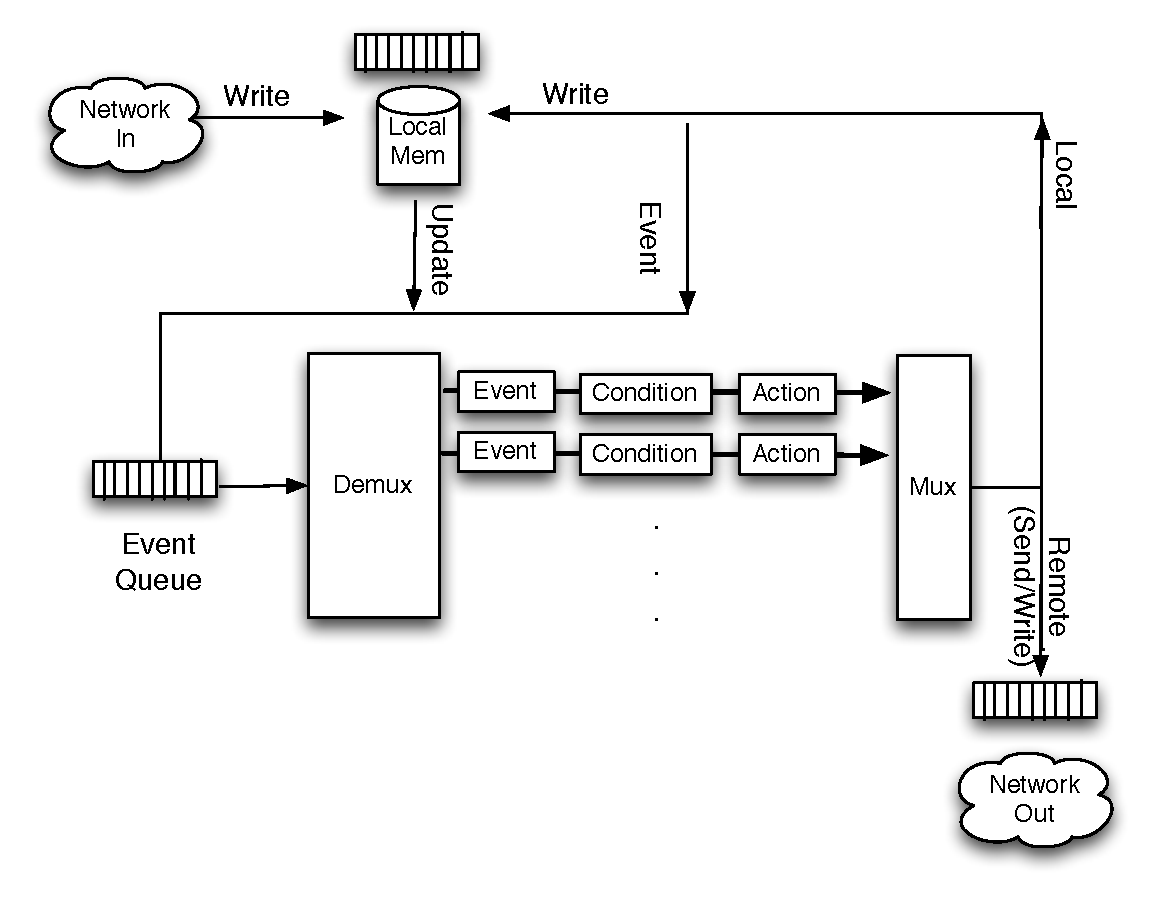
\includegraphics[scale=0.6]{figures/p2-arch}
\caption{\label{ch:p2:fig:dataflow}P2 Dataflow Architecture.}
\end{center} 
\end{figure*}

The P2 architecture consists of a dataflow of processing elements and queues,
and a single driver loop.  Figure~\ref{ch:p2:fig:dataflow} provides a
high-level view (driver omitted) of this architecture, which contains three
queuing elements.  The \ol{event} queue represents the primary input queue,
which contains the current snapshot of tuples that the system uses to drive the
processing.  The \ol{localmem} secondary queue feeds the main event queue with
tuples when none currently exist in it.  Tuples in the \ol{localmem} queue
represent side-affecting events (i.e., insert and delete) to local memory
relations.  P2 evaluates this queue in a tuple at a time fashion, where a
single tuple is dequeued and executed in a ``dataflow fixpoint.''

The P2 architecture contains three output queues that hold the tuples derived
from the rule engine.  The choice of which queue a tuple is added to depends on
the value of the location attribute.  If the tuple's location is local to the
current P2 instance, and its lifetime is greater than zero, then it will be
added to the \ol{localmem} queue.  If the tuple is remote, then it is added to
the \ol{netout} queue.  The third output queue is the \ol{event} queue.  All
(possibly many) local tuples that have a zero-lifetime are directly added to
the event queue, which continues to drive rule deductions until no zero-lifetime
tuples locally exist.  This implementation decision exhibits a kind of
``mini-fixpoint'' (a side-effect unique to P2-\OVERLOG) that we refer to as a
{\em dataflow fixpoint}, which occurs when all tuples in the event queue have
been drained.  We describe this by example.

Assume a single tuple in the \ol{localmem} input queue, and all other queues
are empty.  When the driver executes its ``pull-push'' element on the input of
the empty \ol{event} queue, it will dequeue a tuple in the \ol{localmem} queue
and add it to the \ol{event} queue.  In an iterative loop, the driver will
dequeue a single tuple from the \ol{event} queue and ``route it'' to the
processing elements, which then produce some number of new tuple deductions.
If any of those deductions contain local tuples with a zero lifetime, then they
are reinserted into the \ol{event} queue.  The tuples with non-zero lifetimes
represent ``write'' (insert or delete) actions against the local database (in
\ol{localmem}), and they are (silently) queued while the driver then continues
to process tuples solely from the \ol{event} queue until it is again empty.  At
this point, P2 declares a dataflow fixpoint, which triggers a flush of the
local~\footnote{Write actions from the network input are buffered and applied
at the end of a ``global fixpoint.''} ``insertion'' action writes from the
(silent) queue, generating some number of new event tuples that are added to the
\ol{localmem} queue.  If no ``insertion'' action tuples exist then a flush of
the ``deletion'' action tuples occurs, and the corresponding deletion events
are added (directly) to the \ol{event} queue, before the process repeats, this
time treating deductions as further deletions.

After all insertion and deletion tuples have been processed by the initial
\ol{localmem} input tuple, the system declares a {\em global fixpoint}.  At
this point, the driver loop will flush all tuples in the \ol{netout} queue,
triggering a transfer of those tuples to the corresponding P2 instances
spanning the network.  The driver loop then returns to the \ol{localmem} queue
for the next tuple to process.

From this perspective, the P2 runtime looks quite a bit like an
Event-Condition-Action (ECA) system with a dataflow underneath: {\em events}
are generated by the system clock and network components, while {\em
conditions} are checked via dataflow processing elements, and {\em actions}
initiate outbound network messages and updates to the database.  A driver loop
continuously routes events from the event queue to the ``conditions'' via the
\ol{demux} element in Figure~\ref{ch:p2:fig:dataflow}.  The initial input to
the driver loop is the single tuple at the head of the \ol{localmem} queue.
This sole tuple is the input to the ``current'' fixpoint.  Next, we
describe the elements that implement the {\em condition} and {\em action}
processing logic.

\subsection{Dataflow Elements} 
\label{ch:p2:sec:dataflow_elements}

The set of elements provided in P2 includes a suite of operators familiar from
relational query engines: selection, projection, and in-memory indexes.  These
operators are strung together to implement the logical {\em condition} of the 
processing loop.  P2 supports joins of two relations in a manner similar to the
symmetric hash join: it takes an arriving tuple from one relation, inserts it
into an in-memory table for that relation, and probes for matches in an access
method over the other relation (either an index or a scan).  The work described
in Chapter~\ref{ch:evita} extended this suite to include sorting and
merge-joins, which allowed us to explore some traditional query optimization
opportunities and trade-offs (Chapter~\ref{ch:opt}).

P2 consists of exactly two logical {\em actions}: a local database write and a
network send.  We first describe the details of behind a database write.  An
\ol{event} tuple is modeled as transient database write, and therefore its
action is the reinsertion into the \ol{event} queue.  P2 did not have support
for persistent storage, beyond the ability to read input streams from
comma-separated-value files.  Its tables are stored in memory-based balanced
trees that are instantiated at program startup; additional such trees are
constructed by the planner as secondary indexes to support predicate join
attributes.  A write to the database is applied to the memory-based table, and
a relevant (insert/delete) \ol{event} is enqueued into the \ol{localmem} queue.

The action for a remote output tuple is to simply enqueue it on the \ol{netout}
queue.  When this queue is eventually flushed by the driver loop, all tuples in
it are sent over the network prior to the next fixpoint iteration.  As part of
the same dataflow, P2 provides a number of elements used for networking, which
handle issues like packet fragmentation and assembly, congestion control,
multiplexing and demultiplexing, and so on; these are composable in ways that
are of interest to network protocol designers~\cite{condie-hotnets05}.  The
basic pattern that the reader should assume is that each P2 node has a single
IP port for communication, and the dataflow graph is ``wrapped'' in elements
that handle network ingress with translation of packets into tuples, and
network egress with translation of tuples into packets.

%\subsubsection{Driver Loop}

%We now describe the complete control flow in the P2 runtime.  As mentioned
%above, it is driven by a fairly traditional event loop that responds to any
%network (or timer) event by invoking an appropriate dataflow segment to handle
%the event.
%
%The basic control loop in P2 works as follows:
%\begin{CompactEnumerate}
%    \item An event is taken from the system input queue, corresponding to a single newly-arrived tuple, which is either an {\em insert} tuple (i.e., the result of a normal deduction) or a {\em delete} tuple (the result of a \ol{delete} rule or a primary-key update).  We will refer to this tuple as the {\em current tuple}.
%    \item The value of the system clock is noted in a variable we will call the {\em current time}.  This is the time that will be used to determine the liveness of soft-state tuples.  
%    %(Note that any event tuples that arrived previously will no longer be live in any event table, which guarantees the single-event semantics described above.)
%    \item The current tuple is, logically, appended to its table.
%    \item If the current tuple is an insert tuple, the dataflow corresponding to the \OVERLOG program is initiated and run to a local fixpoint following traditional Datalog semantics, with the following exception: during processing, any non-local derived tuples are buffered in a {\em send queue}, as are any derived tuples to be deleted.
%    \item If, instead, the current tuple is a delete tuple, the dataflow
%    is run to a local fixpoint, but newly-derived local tuples
%    (including the current tuple) are copied to a {\em delete queue},
%    and newly-derived non-local tuples are marked as delete tuples
%    before being placed in the send queue so as to cascade the deletions
%    to remote nodes' databases.
%    \item All tuples in the delete queue are deleted from their associated tables, and the delete queue is emptied.
%    \item The send queue is flushed across the network, with any local updates inserted into the local input queue.
%\end{CompactEnumerate}

%Unlike Datalog, \OVERLOG must run in the continuous processing context of
%networking, over streams of tuples representing system events.  This inherently
%requires more than the single computation of a fixpoint as described in the
%Datalog literature.  P2 has modified its handling of this issue since the
%initial paper~\cite{p2:sosp}.  P2 nests a fairly traditional declarative
%Datalog fixpoint execution within an operationally defined local event loop at
%each node.  An input queue is kept at each P2 node, to hold tuples that
%correspond to network messages and clock interrupts.  Each tuple in the queue
%is tagged with the name of a relation in the schema of the Datalog database.
%The loop begins by noting the local wall-clock time, and deleting from all
%tables any tuples whose soft-state lifetime has expired; this includes event
%tuples from the previous iteration of the loop.  At that point, a tuple is
%dequeued from the input queue and inserted into its associated table.  At that
%point, the \OVERLOG program is run to fixpoint atomically, nearly as if it were
%a traditional single Datalog program.  One exception to traditional Datalog is
%the handling of derived tuples with remote location specifiers; these are
%placed directly into network queues for subsequent processing.  Another
%exception involves rules that have {\em actions} in the head -- these actions
%can be table insertion or deletion; derived tuples in such rules are also
%enqueued for subsequent processing.  When fixpoint is reached, the queued
%network messages are sent to their destinations, and the table actions are
%carried out on the database.  This completes one iteration of the event loop.



% \jmh{This is probably too long.  Also, we need to purge text that was recycled from SOSP.  }
% The design of P2 was inspired by prior work in both databases and
% networking. It is based in large part upon a
% side-by-side comparison between the PIER peer-to-peer query
% engine~\cite{pier-cidr05} and the Click router~\cite{click-tocs}. Like
% PIER, P2 can manage structureddata tuples flowing through a broad
% range of query processing elements, which may accumulate significant
% state and perform substantial asynchronous processing.  Like Click, P2
% stresses high-performance transfers of data units, as well as dataflow
% elements with both ``push'' and ``pull'' modalities. 
% 
% At a coarse grain, P2 in its current state consists of (1) an \OVERLOG
% parser, (2) an Planner that translates \OVERLOG to a runtime dataflow
% plan, and (3) a runtime plan executor.  The
% life of a query is simple: the query is parsed into an internal
% representation, the planner constructs a corresponding dataflow graph
% of elements, and the graph is executed by the runtime until it is
% canceled.  We proceed to overview the components bottom-up; more
% details are given in the P2 SOSP paper~\cite{p2:sosp}.
% 
% Processing in P2 is handled with a dataflow model inspired by Click
% and PIER.  As in Click, nodes in a P2 dataflow
% graph can be chosen from a set of C++ objects called
% \textit{elements}.  In database systems these are often called
% \textit{operators}, since they derive from logical operators in the
% relational algebra.  Elements have some number of input and output
% \emph{ports}.  An arc in the dataflow graph is represented by a
% binding between an output port on one element and an input port on
% another.  Tuples arrive at the element on input ports, and elements
% emit tuples from their output ports. Handoff of a tuple between two elements takes one
% of two forms, \emph{push} or \emph{pull}, determined when the elements
% are configured into a dataflow graph.   
% 
% P2 provides a number of built in dataflow elements that allow it to
% implement networking and query processing logic.  This includes
% elements for the streaming relational query operators found in most
% database systems, e.g., selection, projection, join, and aggregation.
% It also includes networking elements responsible for socket handling,
% packet scheduling, congestion control, reliable transmission, data
% serialization, and dispatch.  P2 has elements to store incoming tuples in tables, 
% iteratively emit tuples in a table matching a filter expression, and {\em listener}
% elements that are notified whenever a tuple is added or deleted from a
% table. Finally, like Click, P2 includes a collection of general-purpose
% ``glue'' elements, such as a queue, a multiplexer, a round-robin
% scheduler, etc.
% 
% Storage in P2 is currently via a main-memory relational Table
% implementation, named using unique IDs that can be shared between
% different queries and/or dataflow elements.  In-memory indices
% (implemented using standard balanced binary trees) can be attached to
% attributes of tables to enable quick equality lookups.  The current
% in-memory implementation serves the system requirements for implementing
% network overlays and streaming query applications, all of which tend
% to expire tuples from memory rather than accumulating them
% indefinitely.  P2's event-driven, run-to-completion model obviates the
% need for locking or transaction support, and relatively simple indices
% suffice to meet performance requirements.  We plan additional
% table implementations that use stable storage for persistent data
% storage; that engineering task is relatively straightforward, but not
% within the scope of this paper.
% 
